\documentclass{article}
\usepackage[left=2cm, right=2cm, top=2cm]{geometry}
%%%%%%%%%%%%%%%%%%%%%%%%%%%%%%%%%% PACKAGES %%%%%%%%%%%%%%%%%%%%%%%%%%%%%%%%%%
\usepackage{minted}                     % Code
\usepackage{graphicx}                   % PNGs
\usepackage{algorithm}
\usepackage{algpseudocode}              % Algorithms
\usepackage{amsmath}                    % Rightarrow
\usepackage{hyperref}                   % Hyperlinks
\hypersetup{
    colorlinks,
    linkcolor=black
}

%%%%%%%%%%%%%%%%%%%%%%%%%%%%%%%%%%%%%%%%%%%%%%%%%%%%%%%%%%%%%%%%%%%%%%%%%%%%%%%

\pagenumbering{gobble}

\title{\textbf{Programming Assignment #2}}
\author{MacMillan, Kyle}
\date{November 12, 2018}


\begin{document}

\maketitle
\addcontentsline{toc}{section}{Title}

\newpage
\pagenumbering{roman}   % Set TOC page numbering to lowercase roman numerals
\tableofcontents
\addcontentsline{toc}{section}{Table of Contents}

\newpage
\listoffigures
\addcontentsline{toc}{section}{List of Figures}

\newpage
\pagenumbering{arabic}  % Set content page numbering to arabic numerals
% Setup Hyperlinks for the rest of the document
\hypersetup{
    colorlinks,
    citecolor=blue,
    filecolor=black,
    linkcolor=blue,
    urlcolor=blue
}

\section{Description of the program}
\setcounter{page}{1} % Set the page counter to 3
 This writeup is for 
 \href{https://www.mcs.sdsmt.edu/ckarlsso/csc410/fall18/csc410_PRG2.pdf}{Programming Assignment #2}.
\\

The program I wrote constructs a class that can test a matrix multiplied with a 
vector and matrix added to another matrix. This was done with a class function 
because there was a lot of repeat code and I like compartmentalizing code. The 
primary functionality of the class is overloaded to accept arbitrary 
matrices/vectors, though they must be of size specified at class instantiation. 

For example you can pass a matrix and vector of your choosing to $AdotBfast$ 
and it will skip the randomization of values, utilizing the arrays you passed 
in.

To use this class simply declare it with the $n$ you intend to use for the $n$ 
$x$ $n$ matrix and $n$ $x$ 1 vector. The class will generate random numbers to 
fill the matrix and vector. If you want to pass it your own matrix and vector 
you can do so by calling the appropriate function with the 1D matrix and vector 
you would like to use. It was done this way because it was very quick to do and 
greatly increases the usage range. 

All public functions, other than sanity check, return the 1D array result, but 
is \textbf{free'd} on the next public function call so it is important to use 
it before you lose it. The program intenionally allocates extra memory because 
I wanted to keep the code clean. Extra memory allocation does not hamper the 
performance testing because I did not include that in the measurement.

When the class is destructed all allocated memory is freed on both the host and 
device.

Users can specify a matrix/vector size or not, the program will run regardless. 
I set a hard limit of matrix/vector size $n$ being 1024. It could have been 
arbitrarily large and increased complexity arbitrarily. This limit was set to 
keep my workload balanced and still produce a detailed writeup and useful 
class.


\section{Description of the algorithms and libraries used}
A $matrix$ x $vector$ has the unique characteristic of applying $one$ number to 
an entire column of numbers. I used this fact to break the parallization into 
two parts. The first part takes the matrix and multiplies each column by the 
associated element in the vector. That data is stored in a matrix. That stored 
matrix is then passed to a secon CUDA function that performs an addition across 
the row. This addition step takes a mere $3us$ on a $1024x1024$ matrix.

For the graduate portion of the assignment I simple pushed everything into a 1D 
array and added things element-wise. There is nothing fancy going on. Each 
addition is allocated to an available core and it is \textbf{incredibly} quick 
as can be seen in Section \ref{sec:test}.

The library used was the CUDA library, so the code for this assignment must use 
the CUDA compiler. $fabs$ was called in one function, so I am also using 
\verb|#include <math.h>|, but that does not require any special compilation 
instructions.


\section{Description of functions and program structure}
See the code under \verb|Prog2.cu|. There are function headers with full 
descriptions for every function. Program flow is:
\begin{enumerate}
    \item fast sanity check
    \item slow sanity check
    \item fast matrx * vector
    \item slow matrx * vector
    \item fast matrix + matrix
    \item slow matrix + matrix
\end{enumerate}
With breakdowns in each function header.


\section{How to compile and use the program}
This program can be compiled with the Makefile. Simply type: \texttt{make p2}

\noindent If you do not have access to the Makefile you can compile it with:
\verb|nvcc -o prog2 Prog2.cu -std=c++11|

\noindent To use the program type: \verb|.\prog2| or \verb|.\prog2 #| 

\noindent where \verb|#| reprsents a number between 1 and 1024.

\newpage
\section{Description of the testing and verification process}{\label{sec:test}}
To test this I began with a sanity check function to ensure I was even 
performing the matrix-vector multiplication as expected. I took a simple 3 $x$ 3 
matrix and multiplied it with a 3 $x$ 1 vector. I verified the output was correct 
and then pressed on. After learning more about CUDA and what was going on I 
determined a 3 $x$ 3 matrix was not sufficient to test. It is too cumbersome to 
come up with a testable $n$ $x$ $n$ matrix of sufficient size so I used the identity 
matrix because $AI = A$ so I was able to easily perform a sanity check where $A$ 
was represented with an ascending number of integers. 

After verifying the correctness of the algorithm I tested the speed of a 
single-threaded version of the algorithm, as can be seen in Figure \ref{fig:slow}.

\begin{figure}[h]
    \centering
    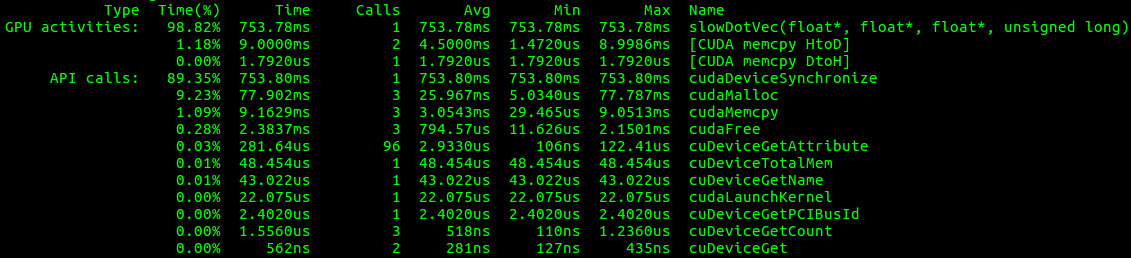
\includegraphics[width=0.95\textwidth]{slow}
    \caption{Single Thread Matrix * Vector}
    \label{fig:slow}
\end{figure}

I then compared that to the fully-parallelized version of the code, as shown in 
Figure \ref{fig:fast}. If we compare the function runtime of the single-threaded 
and multi-threaded functions we see they took $753780us$ and 
$1968.9us + 3.04us = 1971.94us$ respectively. That is a speedup of about $382.5$ 
times faster utilizing the full power of the CUDA cores. We can then calculate 
the Karp-Flatt metrix using $p=1024$ as:

$$e = \frac{\frac{1}{\psi} - \frac{1}{p}}{1 - \frac{1}{p}}$$
$$\frac{1}{\psi} = 0.002616068$$
$$\frac{1}{p} = 0.000976562$$

Which yields a Karp-Flatt metric of:
$$e = 0.001641108$$

\begin{figure}[h]
    \centering
    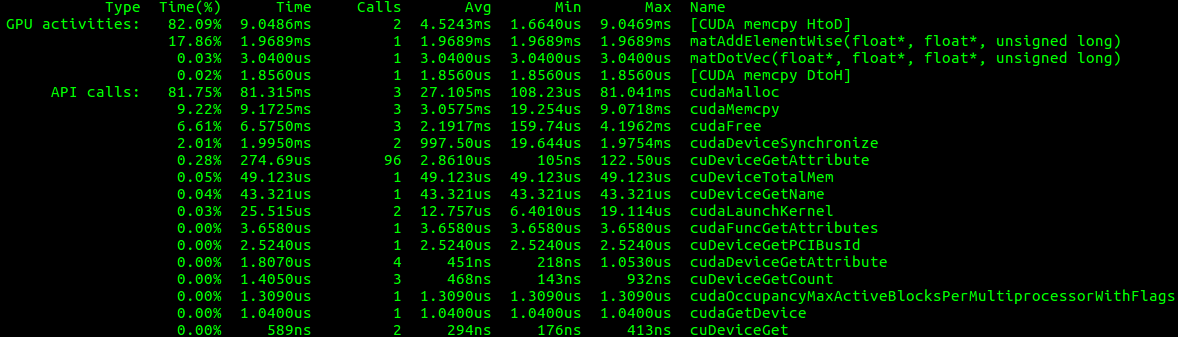
\includegraphics[width=0.95\textwidth]{fast}
    \caption{Multi Thread Matrix * Vector}
    \label{fig:fast}
\end{figure}

For the graduate portion of the assignment you can see the single-threaded 
performance via Figure \ref{fig:slowGrad} and the full parallel implementation 
performance can be seen in Figure \ref{fig:fastGrad}.

\begin{figure}[h]
    \centering
    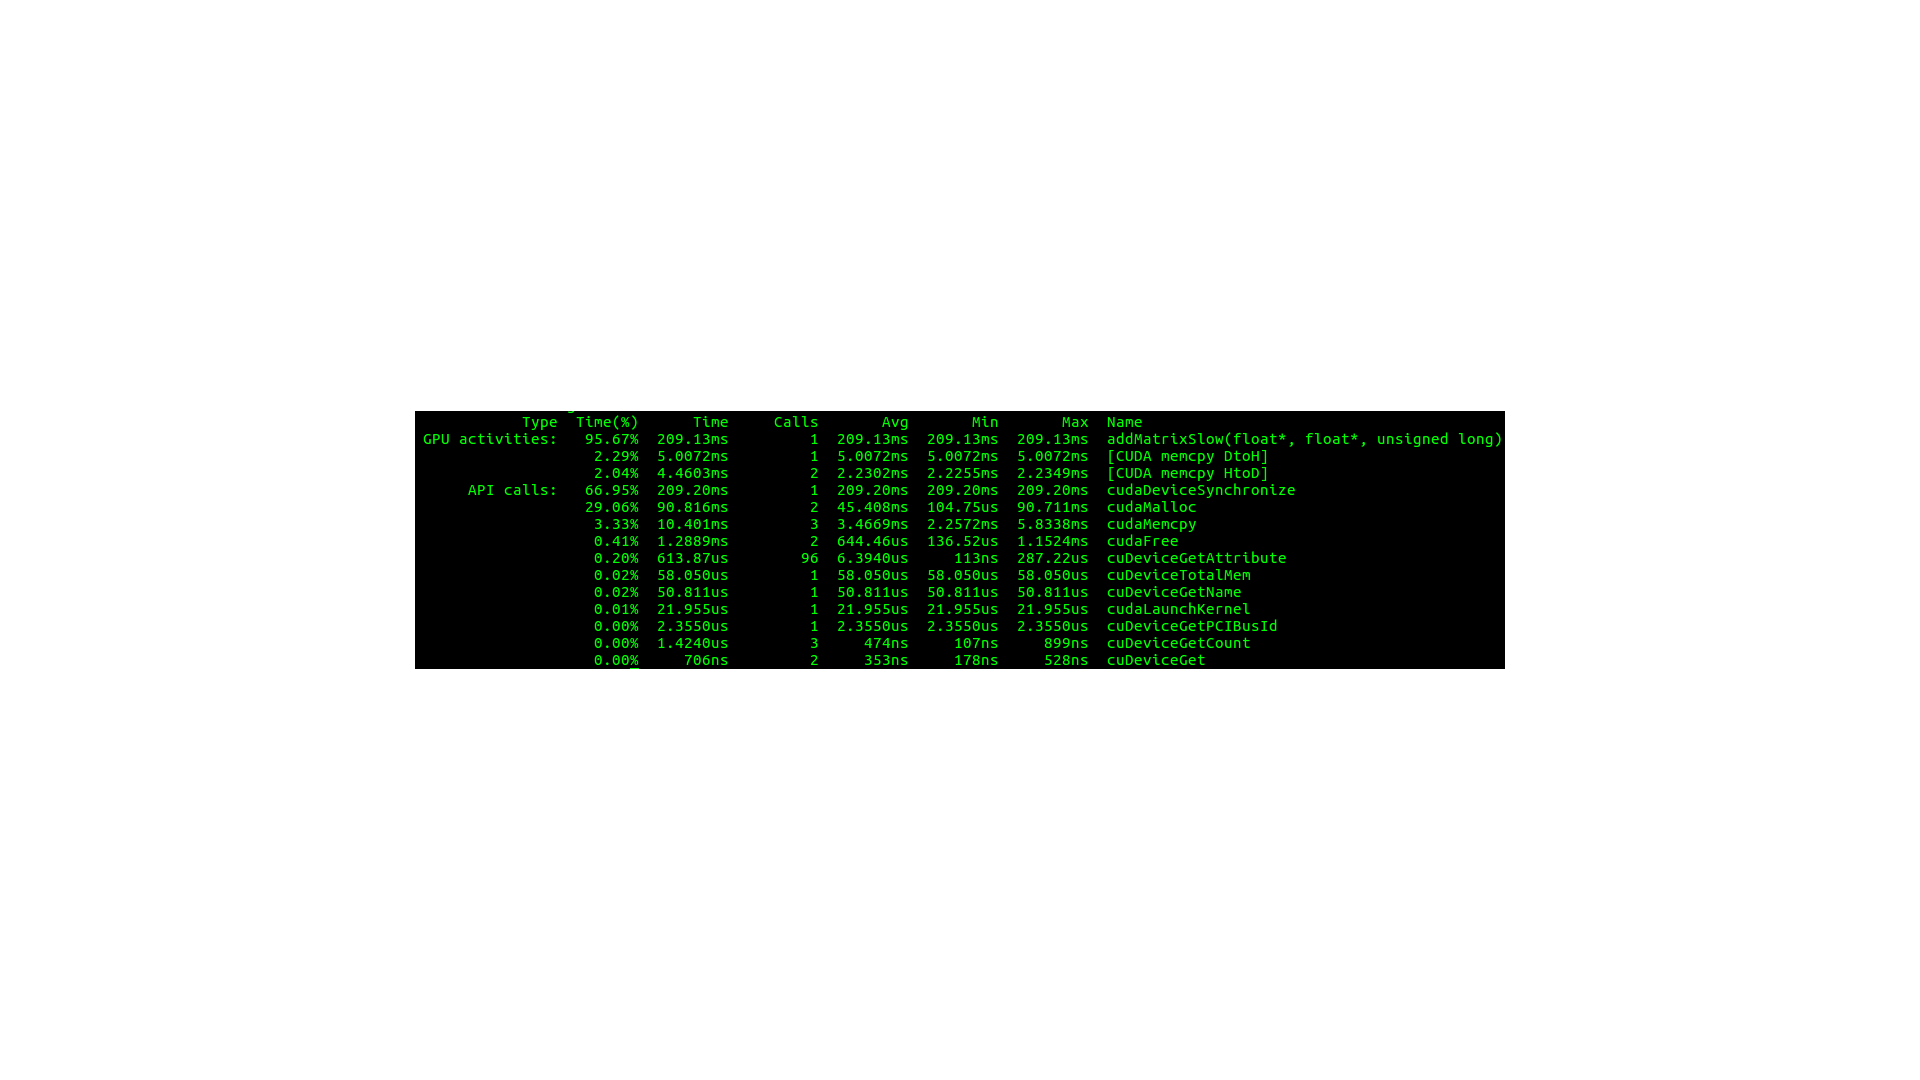
\includegraphics[width=0.95\textwidth]{slowGrad}
    \caption{Single Thread Matrix + Matrix}
    \label{fig:slowGrad}
\end{figure}



\begin{figure}[h]
    \centering
    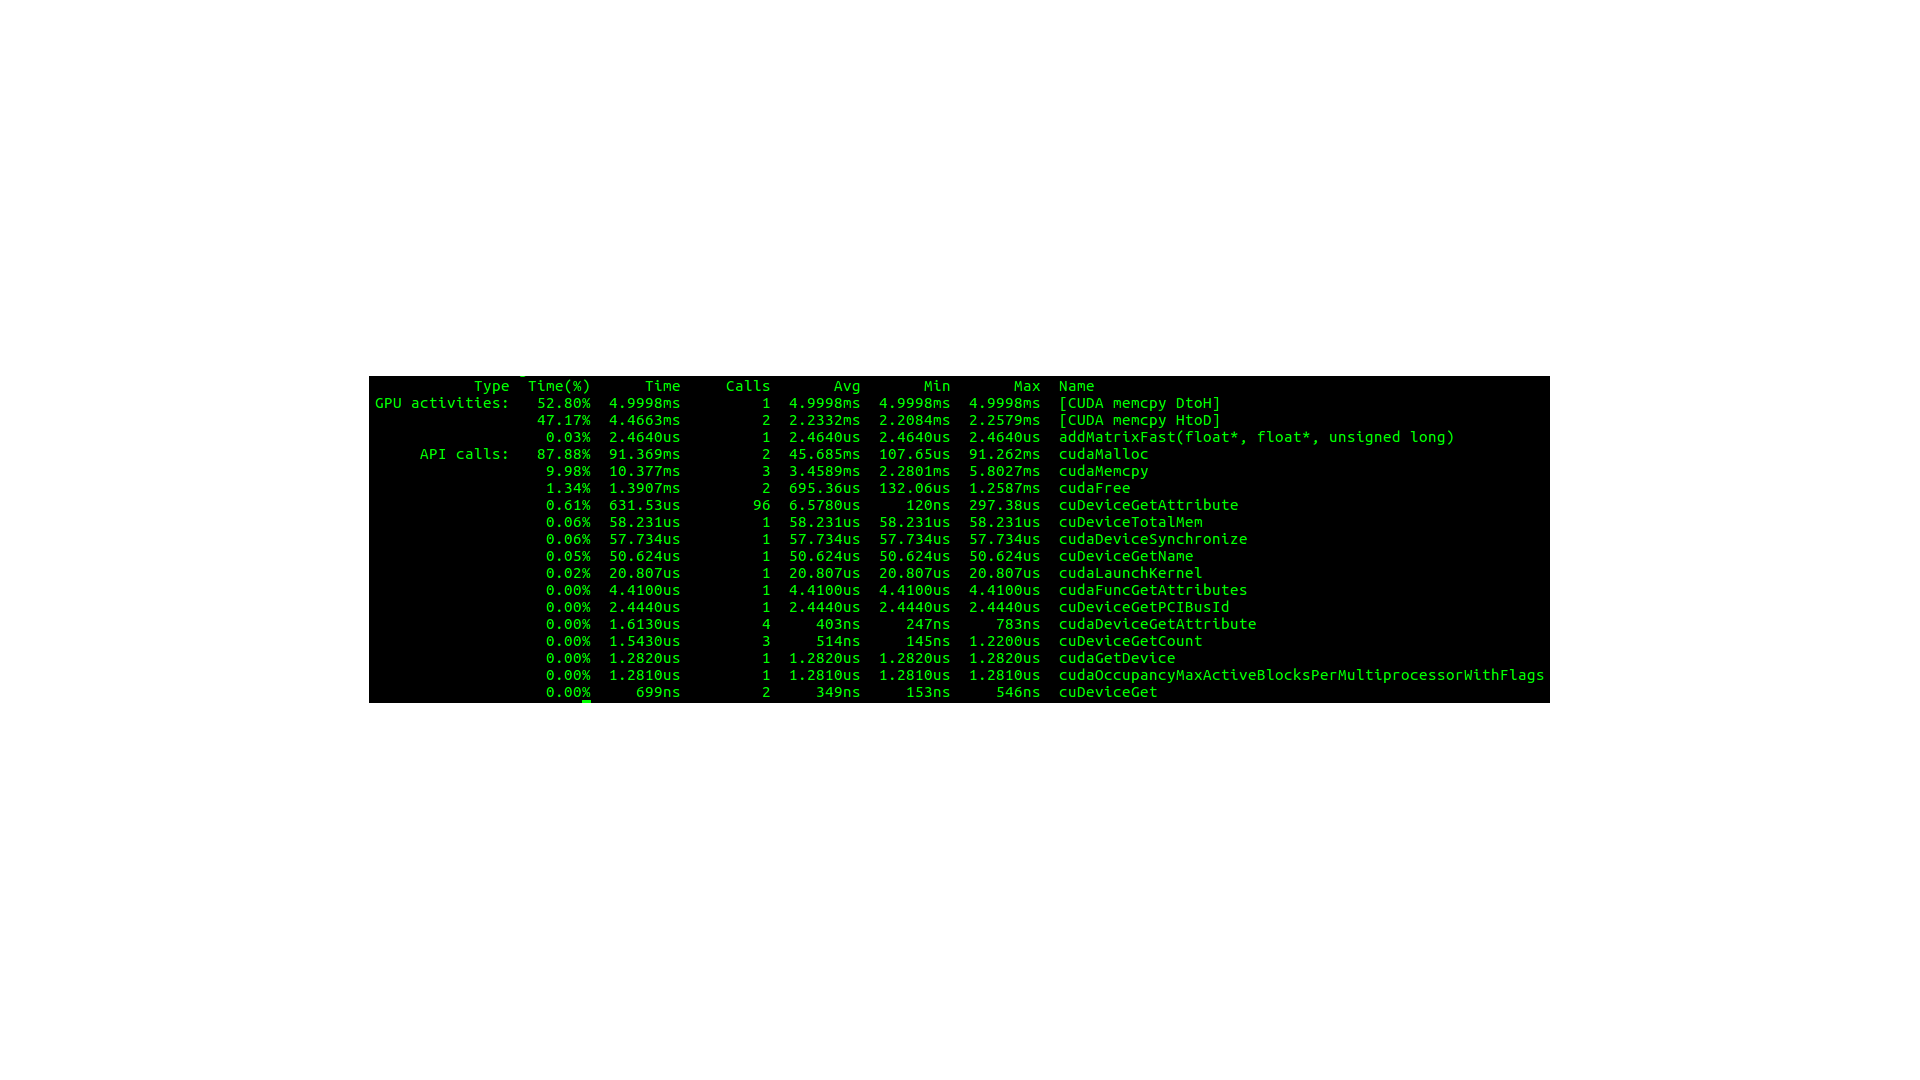
\includegraphics[width=0.95\textwidth]{fastGrad}
    \caption{Multi Thread Matrix + Matrix}
    \label{fig:fastGrad}
\end{figure}

If we compare the runtime of the single-threaded and multi-threaded functions we 
see they took $209130us$ and $2.46us$ respectively. That is a speedup of about 
$85,012$ times faster utilizing the full power of the CUDA cores. We can then 
calculate the Karp-Flatt metrix using $p=1024$ as:

$$e = \frac{\frac{1}{\psi} - \frac{1}{p}}{1 - \frac{1}{p}}$$
$$\frac{1}{\psi} = 0.000011763$$
$$\frac{1}{p} = 0.000976562$$

Which yields a Karp-Flatt metric of:
$$e = -0.000965742$$

At first I believed there was no way it could be a negative number but then I 
realized since we are not taking into account overhead it is in fact possible 
because each operation is 100\% independent of the other operations, it is 
\textbf{fully} parallelizable. If 100\% of the operations are parallelizable and 
overhead is ignored, then it is possible to break this metric. 
\textit{Interesting}.


\section{Description of what you have submitted}
Included in the submission is the code needed to compile the program, a Makefile 
to compile said code, and a detailed writeup of the assignment in pdf form.


\end{document}
